\subsection{MediaPipe Pose}
\label{subsec:mediapipepose}

MediaPipe Pose merupakan salah satu \emph{machine learning solutions} yang dimiliki oleh MediaPipe.
MediaPipe Pose memungkinkan deteksi pose tubuh manusia melalui masukan video RGB menggunakan BlazePose \citep{cit:bazarevsky2020}.
Saat ini deteksi pose yang diproses menggunakan solusi ini mampu menghasilkan performa \emph{real-time} pada perangkat mobile, desktop, dan web.

\begin{figure}[ht]
  \centering
  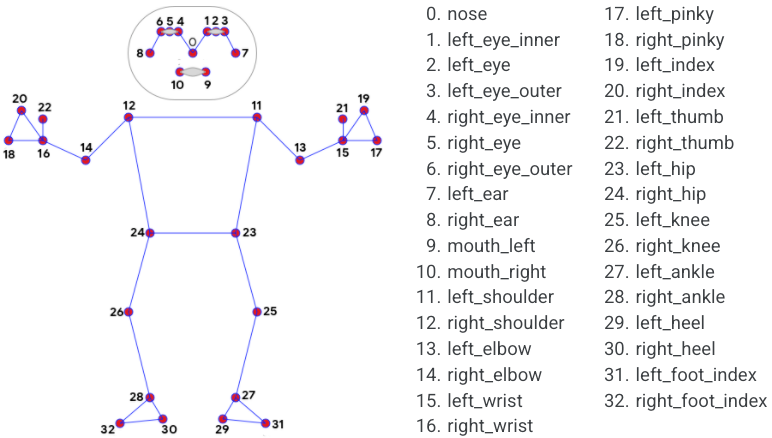
\includegraphics[width=0.95\textwidth,keepaspectratio]{gambar/landmarks-mediapipe-pose.png}
  \caption{Daftar \emph{landmarks} yang ada pada BlazePose \citep{cit:bazarevsky2020}.}
  \label{fig:landmarksmediapipepose}
\end{figure}

Pada MediaPipe Pose,\emph{ pipeline} yang dilakukan adalah pertama dengan menentukan \emph{region-of-intereset} (ROI) dari seseorang atau pose pada suatu \emph{frame}.
Kemudian dari ROI yang dihasilkan, \emph{landmark} untuk setiap bagian dari pose akan dideteksi dan dilacak.
Seperti yang terlihat pada gambar \ref{fig:landmarksmediapipepose},
  terdapat total 33 \emph{landmarks} yang dihasilkan oleh proses deteksi ini.
\emph{Landmarks} tersebut terdiri atas setiap bagian yang ada pada pose manusia.
Dari proses tersebut, hasilnya adalah daftar \emph{landmarks} yang terdeteksi beserta koordinat dari masing-masing \emph{landmark} dalam ruang 3D.
